\newpage
\subsubsection{Creating EReferences in EA}
\visHeader
\hypertarget{static:references vis}{}

\begin{itemize}

\item[$\blacktriangleright$] A fundamental gesture in EA is \emph{Quick Link}. Quick Link is used to create references between elements in a context-sensitive
manner. To use Quick Link, choose an element and note the little black arrow in its top-right corner (Fig.~\ref{fig:quicklink}).

\begin{figure}[htbp]
	\centering
  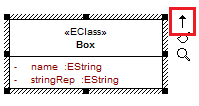
\includegraphics[width=0.4\textwidth]{ea_quickLink}
	\caption{Quick Link is a central gesture in EA}
	\label{fig:quicklink}
\end{figure}
\FloatBarrier

Click this black arrow and `pull' to the element you wish to link to. To start, quick-link from \texttt{Box} to \texttt{Partition}. In the context menu
that appears, select ``Create Bidirectional EReference'' (Fig.~\ref{fig:ereference}).

\begin{figure}[htbp]
	\centering
  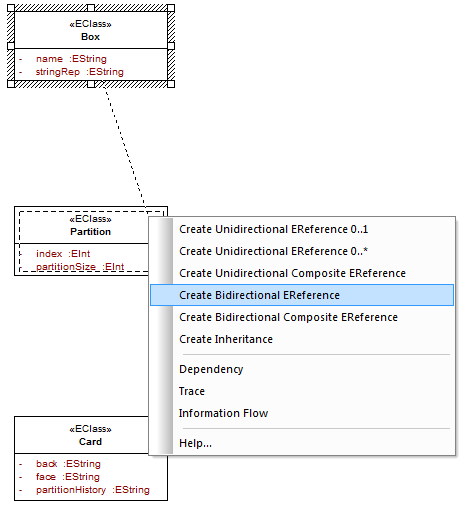
\includegraphics[width=0.6\textwidth]{ea_eReferenceBidirectional}
	\caption{Create a reference via Quick Link}
	\label{fig:ereference}
\end{figure}
\FloatBarrier

\item[$\blacktriangleright$] Double click the reference to invoke a dialogue. Here you can switch the reference from bi-direction to a uni-direction, change the
source and target classes, and enter a name. Feel free to leave the \texttt{Name} value blank - this property is only used for documentation purposes, and not
relevant to code generation.

\item[$\blacktriangleright$] Within this dialogue, go to ``Target Role'', and enter the values in Fig.~\ref{fig:role_target} to set the properties for the
\emph{Target} end of the reference (the \texttt{Box} role). As you can see, the default target is set to the class you linked \emph{from}, and the default
\emph{Source} is the class you linked \emph{to}. In this window, it's important not to forget to confirm and modify the \texttt{Role}, \texttt{Navigability},
\texttt{Multiplicity}, and \texttt{Aggregation} settings for the target.  Repeat the process for the \texttt{Source Role} (Fig.~\ref{fig:role_source}).

\vspace{0.5cm}

\item[$\blacktriangleright$] If you decided to ignore the previous instructions, and went from \texttt{Partition} to \texttt{Box}, the only difference between
what you see here versus on your screen is a reversal of roles. The following information will still be the same! You can switch the roles by returning to the 
``General" window and modifying \texttt{Target} and \texttt{Source} there. 
\vspace{1cm}

\begin{figure}[htbp]
	\centering
	  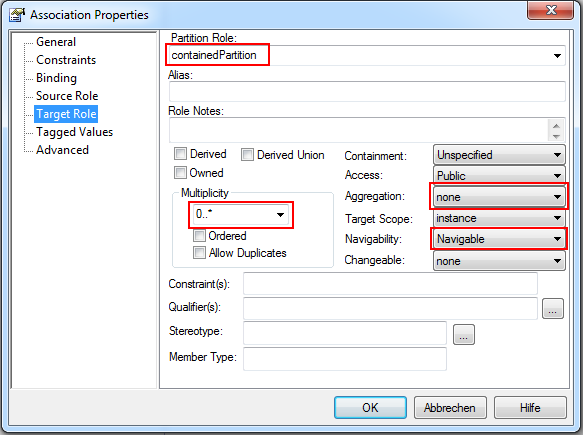
\includegraphics[width=0.9\textwidth]{ea_assocPropsTarget}
	\caption{Properties for the target role of a reference}
	\label{fig:role_target}
\end{figure}
\FloatBarrier

\begin{figure}[htbp]
	\centering
    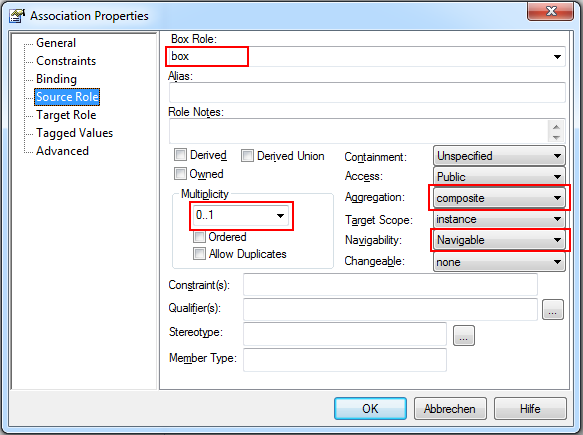
\includegraphics[width=0.9\textwidth]{ea_assocPropsSource}
	\caption{Properties for the source role of a reference}
	\label{fig:role_source}
\end{figure}
\FloatBarrier

\end{itemize}

To explain these property windows, the first value you completed was the navigation name. The \texttt{Navigation} value should have been automatically set to
\texttt{Navigable}. Without these, correct getter and setter methods could not be generated.

\vspace{0.5cm}

Next, you set the \texttt{Multiplicity} value. In your target role (\texttt{Box}), you have allowed the creation of up to
one target (\texttt{box}) reference for every connected source (\texttt{Partition}). This means you could not have a single source connected to two targets
(ie., one partition that belongs to two unique boxes). In the source (\texttt{Partition}) role, you have specified that any target (in our case, \texttt{box})
can have any positive-sized number of sources. Figure~\ref{fig:sketch_roles} sketches this idea.

\begin{figure}[htbp]
	\centering
    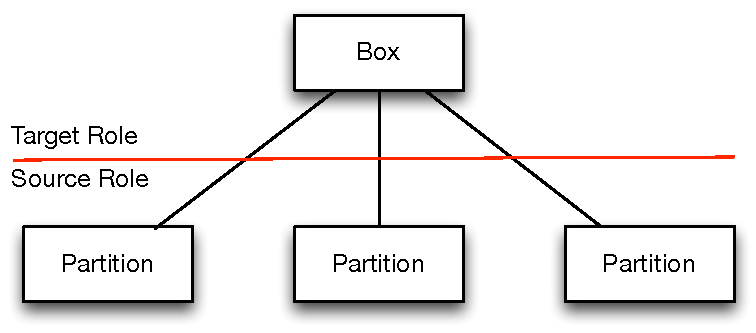
\includegraphics[width=0.6\textwidth]{sketch_multiplicities.pdf}
	\caption{The target and source roles of Leitner's Learning Box}
	\label{fig:sketch_roles}
\end{figure}
\FloatBarrier

Finally, you set the \texttt{Aggregation} value. In this case, \texttt{box} is a
container for \texttt{Partition}s, and \texttt{containedPartition} doesn't need to adhere to any rules.

\begin{itemize}

\item[$\blacktriangleright$] Take a moment to review how the \texttt{Aggregration} settings extend the \texttt{Multiplicity}. If you've done everything right,
your workspace should now resemble Fig.~\ref{fig:ereference_completed}, with a single \emph{Bidirectional EReference} between \texttt{Box} and \texttt{Partition}.

\vspace{1cm}

\begin{figure}[htbp]
	\centering
  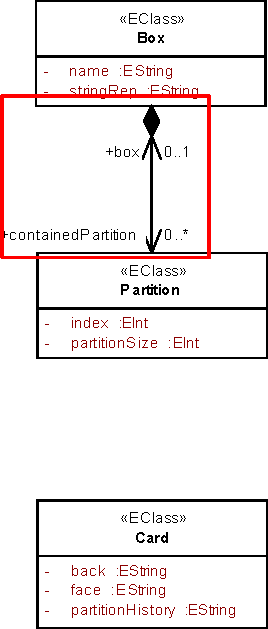
\includegraphics[width=0.4\textwidth]{ea_relationBoxPartition.pdf}
	\caption{\texttt{Box} contains \texttt{Partition}s}
	\label{fig:ereference_completed}
\end{figure}
\FloatBarrier

\clearpage

\item[$\blacktriangleright$] Following the same process, create another bidirectional EReference\footnote{To be precise, \emph{all} references in Ecore are
actually unidirectional.
A ``bidirectional'' reference in our metamodel is really two mapped \texttt{EReferences} that are opposites of each other.
We however, believe it is simpler to handle these pairs as single references, and prefer this concise concrete syntax.} between \texttt{Partition} and
\texttt{Card}, then two unidirectional self-references for \texttt{Partition}. Your final workspace should resemble Fig.~\ref{fig:ereferences_all}.

%explain why we've created this series of relations? (ie: review)

\vspace{1cm}

\begin{figure}[htbp]
	\centering
  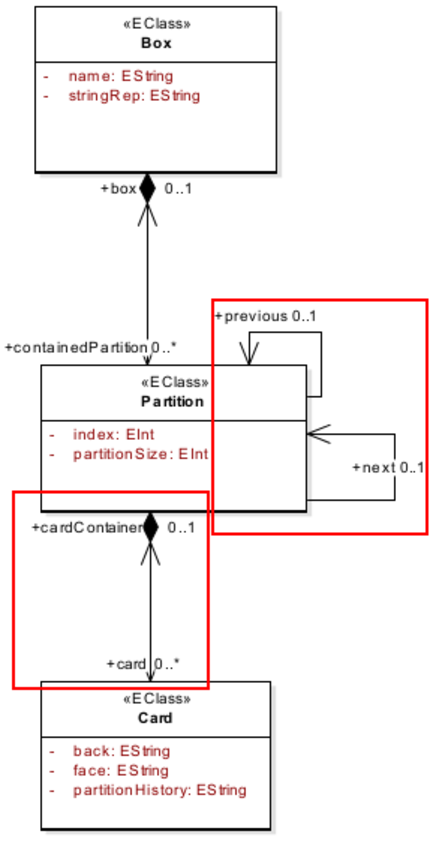
\includegraphics[width=0.6\textwidth]{ea_classAttributes}
	\caption{All relations in our metamodel}
	\label{fig:ereferences_all}
\end{figure}

\FloatBarrier

\item[$\blacktriangleright$] All the attributes and references required for your learning box have now been set up. We encourage you to discover how these are
declared in the textual syntax, in the next section. In particular, check out Fig.~\ref{fig:allReferences}, the classes fully declared with all references.

\item[$\blacktriangleright$] As always, export to Eclipse and refresh your \texttt{Specifications} node.

\fancyfoot[R]{$\triangleright$ \hyperlink{static:methods vis}{Next}}

\end{itemize}
